\makeheading{我是第一篇文章的标题}
\begin{multicols}{3}
    这是一篇文章,它会教你排版。我已经为Interstellar写好了一份文档模板,你只要按照上面的排版流程新建文件就可以了。下面的文字会教你详细的LaTeX排版方式。
    
    看到上面的begin命令了吗?这是开始进行双栏排版的标志。到了该分段的时候,我们要在两段之间插入一个空行。
    
    看到了吗?上面有一个空行,我们成功地分了段!系统会自动帮你加开段的空格!
    
    重要的事情我们不说三遍,只需要告诉系统:\qiangdiao{我要强调!}就好啦,看到了吗?在最终的结果中,“我要强调!”四个字被用蓝色、粗体显示。
    
    好的文章还有图片,图片可以被插在本栏中:只需要在“end{multicols}”命令之前插入:
    
    \begin{figure}[H]
        \centering
        
\includegraphics[width=\linewidth]{IMG/202001/pjtw.jpg}
        \caption{\textit{这里写上对图片的注释——我是一个单栏图片,你会看到我已经被自动标上了序号}}
    \end{figure}
    
    千万不要忘了{figure}后面的“[H]”,否则在双栏环境中图片不会显示。
    
    对于过宽的图片,我们可以跨栏排印,只需要在end命令之外加入上面的几行命令,然后下面再接一个begin命令,就可以继续排印文字了。
    
    准备好了吗?我们要退出双栏环境咯
    
    3,2,1,准备!
\end{multicols}
    
\begin{figure}[H]
    \centering
    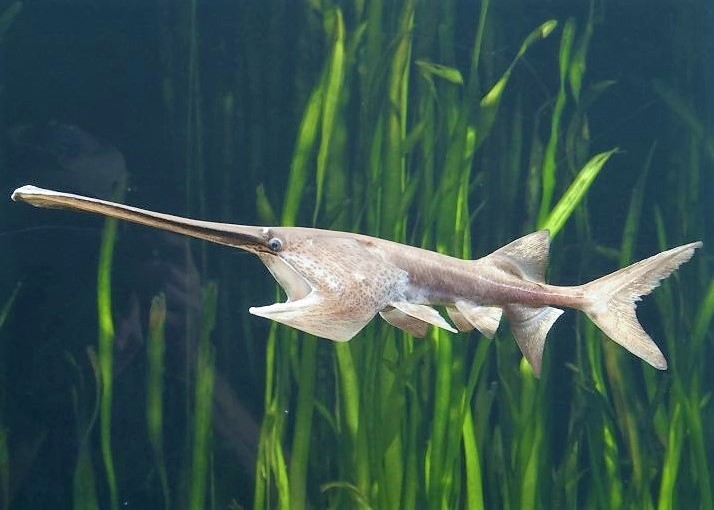
\includegraphics[width=0.6\linewidth]{IMG/202001/cjbx.jpg}
    \caption{\textit{这里写上对图片的注释——我是一个三栏图片,[H]用来告诉电脑:你必须把图片放在这里,否则图片会乱跑}}
\end{figure}
    
\begin{multicols}{3}
    我们又成功进入了三栏环境!
    
    小标题也是一个排印的要素哦,看到那个用灰色框框起来的,蓝色粗体显示的稍大点的字了吗?
    \section*{我就是那种标题哦}
    有的时候还有更小的无框标题,用在科技快讯中:
    \subsection*{我比我大哥小一点}
    千万不要落下那个星号,要么标题就带上了序号,在这种文章中序号可有可无。
    
    到这里,第一篇文章结束了,到了参考文献和广告时间。noindent命令用于使该行不空两格开段,url命令用于使很长的网址正确换行。退出双栏环境后这样就好了:
\end{multicols}

\noindent\qiangdiao{参考文献}

\noindent\url{[1]http://zheshiyige.wangzhi.com}

\ADyixuehui

\newpage

\makeheading{我是第二篇文章的标题}

\begin{multicols}{3}
    \greyboxNID{\qiangdiao{导读\ }第二篇文章就没什么可以说的了,我们刚刚完成了插入广告、换新页,并且插入了标题。看,这是一个导读,用窄边框的灰色盒子包着,只要输入greyboxNID命令再用大括号包住内容就可以了。}
    
    要使文章中的文字斜体,请\textit{斜体文字}。由于汉字字体的斜体比较丑,在本系统中,斜体汉字被变成了楷体的正体字。
    
    关于人名,人民出版社的《学术著作出版规范》有如下建议:按名从主人的原则,翻译成中文,两个单词的翻译之间用“·”隔开,缩写词后用句点“.”。在第一次出现时后面括号加注原名,字体不需要做改变,如:
    
    \begin{enumerate}
        \item 伟大的革命导师卡尔·马克思(Karl Marx)所著的《资本论》全球闻名。
        \item J.K.罗琳(J.K. Rowling)创作的《哈利波特》系列已被改编为电影在全球上映。
    \end{enumerate}
    
    在上面的例子中,你可以看到编号列表的使用方法,如果只需要非编号列表(每项开头用圆点),把“enumerate”改为“itemize”即可。
    
    作为一份科技报刊,怎么能没有公式呢?如果要在行文中插入inline的公式,只需要$E=mc^2$就好啦,如果是那种很长的公式,可以向下面这个向心加速度公式学习:
    \[
    a_n=\frac{v^2}{r}=\omega^2 r=\omega v=\frac{4\pi^2 r}{T}=4\pi^2rf.
    \]
    这个公式被居中在一个新行中显示,从上面的例子中,你会学习到如何上下标,如何输入分式,特殊符号的命令表你可以不必背。
    
    第二篇文章也结束了。如果下面空着很大的地方,那么咱插入一个生活中的科学这样的板块吧:
\end{multicols}

\noindent\qiangdiao{参考文献}

\noindent\url{[1]http://zheshiyige.wangzhi.com}

\greybox{\vskip-25pt
    \makeheading{生活中的科学}
    
    注意在灰盒子命令里使用标题命令时需要加一个“vskip-25pt”命令来消除大片空行。
    
    {\centering
        看到了吗?我已经被居中了!
    }
}
